% TODO methontology is top-down
\chapter{Methodologies for developing ontologies}
\label{ch:development_approaches}

There are numerous methodologies for building ontologies. As this chapter points out, all of them strive for avoiding common pitfalls and try to minimize the need for refactorization at late development steps. Each approach forces the ontology designer to determine as many details about the ontology's domain as early as possible.

% TODO citation: competency questions?
All methodologies have in common that knowledge acquisition is centered around \emph{competency questions} that roughly define a scope for the ontology and details about that scope. Competency questions are stated at the very beginning of the design process and provide the basis for all further steps towards the ontology. The ontology can be considered complete if it is able to provide answers to all competency questions (except the ones that cannot be answered by an ontology).

In the article about their approach towards ontology design, Noy and McGuinness state three fundamental rules~\cite{Ontology101} of ontology design. Although the authors only apply them to their own approach, they hand out advice for many design decisions, regardless of which approach is used for the design of the ontology:

\begin{quote}
\itshape
1) There is no one correct way to model a domain -- there are always viable alternatives. The best solution almost always depends on the application that you have in mind and the extensions that you anticipate.

2) Ontology development is necessarily an iterative process.

3) Concepts in the ontology should be close to objects (physical or logical) and relationships in your domain of interest. These are most likely to be nouns (objects) or verbs (relationships) in sentences that describe your domain.\normalfont\cite{Ontology101}
\end{quote}

This chapter discusses some existing methodologies for the construction of ontologies. Among the methodologies that can be found in literature, the ones discussed as candidates for the design of \thinkhomeweather are

\begin{itemize}
  \item \emph{Ontology 101} by Noy and McGuinness~\cite{Ontology101} (section \ref{subsec:approach1}),

  \item the software enginering approach by De Nicola, Missikoff and Navigli \cite{SoftwareEngineeringOntology} (section \ref{subsec:approach2}),
  
  \item the one by Uschuld and King~\cite{UscholdKing} (section \ref{subsec:approach3}),
  
  \item the one by Grüninger and Fox~\cite{GruningerFox} (section \ref{subsec:approach4}), and
  
  \item \methontology by Gómez-Pérez et al.~\cite{Methontology} (section \ref{subsec:approach5}).
\end{itemize}

There are several other methodologies that are not covered here, such as \emph{Model Driven Ontology}~\cite{ModelDrivenOntology}, the \emph{NeOn Methodology}~\cite{NeOnMethodology}, the approach of Berneras et al. in the context of the \emph{Esprit KACTUS project}~\cite{KACTUSMethodology}, the methodology based on the \emph{SENSUS ontology}~\cite{SENSUSMethodology}, and a method~\cite{FCAMethod} based on \emph{Formal Concept Analysis}~\cite{FormalConceptAnalysis}.

\section{Evaluating ontology development methodologies}

The evaluation in this chapter is loosely based on the article by Fernández-López that evaluates a set of methodologies for building ontologies~\cite{MethodologyOverview}. There are several other articles that cover this topic~\cite{MethodologyComparison1,MethodologyComparison2,MethodologyComparison3}.

For each methodology, the following topics are discussed in section~\ref{sec:ontology_approaches}:

\begin{itemize}
  \item \textbf{Description:} Each step of the methodology is presented.
  
  \item \textbf{Applications:} Some ontologies that have been developed using the methodology are enumerated, if any. Applications may include both cases where the methontology was just applied to provide detailled insights into the methodology itself and cases where the methodology was used for the development of an ontology as part of a project.
  
  \item \textbf{Analysis:} The methodology is analysed regarding a pre-defined set of criteria (see below):
    \begin{itemize}
      \item \textbf{Effort:} Different approaches lead to different efforts for the development of ontologies. Although the minimisation of the effort is not a target of \thinkhomeweather, it is unnecessary to apply an approach which leads to an enormous development effort compared to other methodologies.
      
      \item \textbf{Usage:} If an approach is widely used, this may indicate that the approach is considered suitable for ontology development by many designers. The other way, a seldomly applied methodology may be inappropriate for most use cases.
      
      \item \textbf{Applicability:} An approach may be limited to certain kinds of domains and be unsuitable for designing \thinkhomeweather.
      
      \item \textbf{Strictness:} Due to the fact that there is no one correct way to design an ontology, every approach must leave a certain margin to the ontology designer to decide about implementation details. However, a margin being too wide may lead to an inaccurate or incomplete ontology.
      
      \item \textbf{Documentation:} Methodology may enforce the creation of documentation while others delegate the decisions about how the documentation is structured and what is documented to the ontology designer. This may lead to missing, inaccurate, or incomplete documentation.
    \end{itemize}
\end{itemize}

Section~\ref{sec:approaches_summary} then compares the methodologies with each other while section~\ref{sec:approaches_conclusion} concludes about the results and comes to a decision regarding the methodology which fits the requirements of \thinkhomeweather best and thus will be used for the development of the ontology. It is possible that this decision is not be unambiguous if more than one approach turns out to be suitable for the present context.

As section~\ref{sec:ontology_approaches} focuses on the characteristics of the methodologies required to take a decision in favour of one of the approaches, section~\ref{sec:methontology} then describes the selected approach in a more detailed manner.

\section{The ontology development approaches}
\label{sec:ontology_approaches}

\subsection{Ontology 101}
\label{subsec:approach1}

\subsubsection{Description}

In their paper \emph{Ontology Development 101: A Guide to Creating Your First Ontology}\cite{Ontology101}, Noy and McGuiness present an informal and rather intuitive approach for building ontologies from scratch. It is geared towards people without or with little prior knowledge about how to design an ontology and qualifies for demonstrating the essence of ontologies.

The approach is divided into a set of steps:
\begin{enumerate}
  \item The domain and scope of the ontology are determined. The preferred way for this is to formulate \emph{competency questions} the ontology should be able to answer.
  \item Existing ontologies are considered to be reused to avoid doing work that has already been done and to simplify interoperability with other ontologies.
  \item Important terms in the ontology are enumerated, i.e. a \emph{glossary of terms} is built.
  \item From the glossary in the previous step, all terms that are classes are identified. They are then related to each other in order to create a \emph{class hierarchy}.
  \item The next step iterates all classes and tries to identify terms from the glossary which are properties of the classes.
  \item Then, for the properties the ranges of possible values are specified.
  \item Finally, instances from the glossary are selected and added to the ontology.
\end{enumerate}

\begin{figure}
\centering
\includegraphics[width=\textwidth]{figures/ontology101_process.pdf}
\caption{The workflow proposed by \emph{Ontology 101}.}
\label{fig:ontology101_process}
\end{figure}

These steps are not strictly performed one after the other; instead, an iterative process is proposed which iterates the whole set of steps repeatedly. Figure~\ref{fig:ontology101_process} depicts the workflow this process.

Besides the approach itself, \emph{Ontology 101} provides a huge set of rules of thumb which guide the ontology designer towards a well-conceived ontology, advises her of common pitfalls and help her identify both adequate and improper patterns.

\subsubsection{Applications}

Applications of \emph{Ontology 101} include a \emph{Human Community Ontology}~\cite{HumanCommunityOntology}, an \emph{Ontology for Intrusion Detection}~\cite{IDSOntology}, and an ontology which is part of \emph{BioPAX}, an effort towards improving knowledge exchange in the research of biological pathways~\cite{BioPAX}.

\subsubsection{Analysis}

\emph{Ontology 101} provides a simple and coherent approach for building ontologies. However, it comes with a few downsides.

\begin{itemize}
  \item \textbf{Effort:} The effort of applying \emph{Ontology 101} to a certain domain can be considered to be low.
  
   \item \textbf{Usage:} The methodology is very often cited in literature to give readers an understanding of the basics of ontology development. However, compared to other methodologies, the number of applications is low.
  
  \item \textbf{Applicability:} \emph{Ontology 101} does not state any limitations regarding the use of its approach for arbitrary domains.
  
  \item \textbf{Strictness:} The approach does not enforce strict rules and leaves a broad margin to the ontology designer.
  
  \item \textbf{Documentation:} \emph{Ontology 101} completely lacks a description on how documentation is generated; this may lead to missing, incomplete, or inaccurate documentation.
\end{itemize}

\subsection{A software engineering approach to ontology building}
\label{subsec:approach2}

\subsubsection{Description}

% TODO

\subsubsection{Applications}

% TODO

\subsubsection{Analysis}

% TODO

\subsection{Methodology by Uschold and King}
\label{subsec:approach3}

\subsubsection{Description}

% TODO

\subsubsection{Applications}

% TODO

\subsubsection{Analysis}

% TODO

\subsection{Methodology by Grüninger and Fox}
\label{subsec:approach4}

\subsubsection{Description}

% TODO

\subsubsection{Applications}

% TODO

\subsubsection{Analysis}

% TODO

\subsection{METHONTOLOGY}
\label{subsec:approach5}

\subsubsection{Description}

% TODO

\subsubsection{Applications}

% TODO more details?
Applications of \methontology include the \emph{Legal Ontology}~\cite{MethontologyLegal}, the \emph{Chemical Ontology}~\cite{MethontologyChemical}, the \emph{Graduation Screen Ontology}~\cite{GraduationScreenOntology}, the \emph{Ontology for Metabolic Pathways}~\cite{MetabolicPathways}, the \emph{Vehicles' Ontology} for checking the consistency of official documents in eGovernment~\cite{VehiclesOntology}, the ontology for a context-aware semantic approach for the effective selection of an assistive software~\cite{AssistiveSoftware} and a cartographic ontology~\cite{CartographicOntology}. Some ontology designers opted for an approach that combines \methontology with another approach, e.g. for the development of an educational ontology~\cite{EducationalOntology} using a combination of \methontology and a Model Driven Approach~\cite{ModelDrivenApproach}.
For the development of an ontology in the hydrographical domain~\cite{HydrographicalOntology}, the designers combined the top-down approach of \methontology with a bottom-up approach based on \emph{Formal Concept Analysis}~\cite{FormalConceptAnalysis}.

\subsubsection{Analysis}

% TODO
% \subsection{Combined approaches}

% Some ontology designers opted for development approaches that combined two 

\section{Summary}
\label{sec:approaches_summary}

\section{Conclusion}
\label{sec:approaches_conclusion}

The previous chapters gave detailed insights into some popular approaches of developing ontologies from scratch. Table ? summarizes some of the key charasteristics of these approaches.

% TODO insert table

Considering the characteristics of the development approaches, \methontology was chosen for building the \thinkhomeweather ontology. Thus, \methontology was discussed more thoroughly than the other approaches. The main reasons for that decision were:

% TODO
\begin{itemize}
  \item Some reason.
  \item Some more reason.
  \item And yet another reason.
\end{itemize}

Chapter \ref{ch:thinkhomeweather_ontology} describes the process of building the \thinkhomeweather ontology in detail.

\section{\methontology}

As section~\ref{sec:approaches_conclusion} opted for \methontology as the methodology to be used for developing \thinkhomeweather, this section presents \methontology in a more detailed manner.

\vspace{1em}

The inventors of \methontology, Gómez-Pérez et al., perceived absence of a clear engineering approach towards building ontology from scratch. Hence, they described a process for developing ontologies and specified a life cycle for ontologies. Based upon that, they specified \methontology as a straight-forward engineering approach for building ontologies~\cite{Methontology}.

Several papers describe \methontology itself~\cite{Methontology,Methontology2,ORSD}, while others discuss applications of \methontology in the development of ontologies~\cite{MethontologyLegal,MethontologyChemical}.

While the overall approach is the same in all of these articles, there are slight differences regarding the details of each step. For developing the \thinkhomeweather ontology in chapter \ref{ch:thinkhomeweather_ontology}, a variant of \methontology is used that combines aspects from several papers. This methodology is presented in this section. It does not exactly match the methodology presented in any of the papers.

% TODO mention IEEE software life cycle paper referenced in \cite{MethontologyLegal}?


\subsection{Ontology development process and life cycle}

The ontology development process used by \methontology divides ontology development into the following activities that need to be performed \cite{Methontology}:

\begin{itemize}
  \item \textbf{Planification:} This step involves creating a plan regarding which tasks need to be done, how they will be arranged and which resources they require.
  \item \textbf{Specification:} The purpose, intended uses and end-users are specified in an \emph{Ontologies Requirements Specification Document}.
  \item \textbf{Knowledge acquisition:} Knowledge about the ontology's domain is acquired.
  \item \textbf{Conceptualization:} The knowledge previously acquired is conceptualized into a conceptual model that describes the problem that shall be solved by the ontology and how the ontology solves it.
  \item \textbf{Formalization:} This conceptual model is then formalized.
  \item \textbf{Integration:} As ontologies are built to be reused, as many existing ontologies as possible are integrated into the new ontology.
  \item \textbf{Implementation:} The ontology is then implemented using a formal language.
  \item \textbf{Evaluation:} Throughout the process of building the ontology, it is continuously evaluated in order to ensure it meets the requirements specified previously.
  \item \textbf{Documentation:} The ontology and all documents belonging to it must be well documented.
  \item \textbf{Maintenance:} It may be necessary to apply modifications throughout the lifetime of the ontology.
\end{itemize}

\begin{figure}
  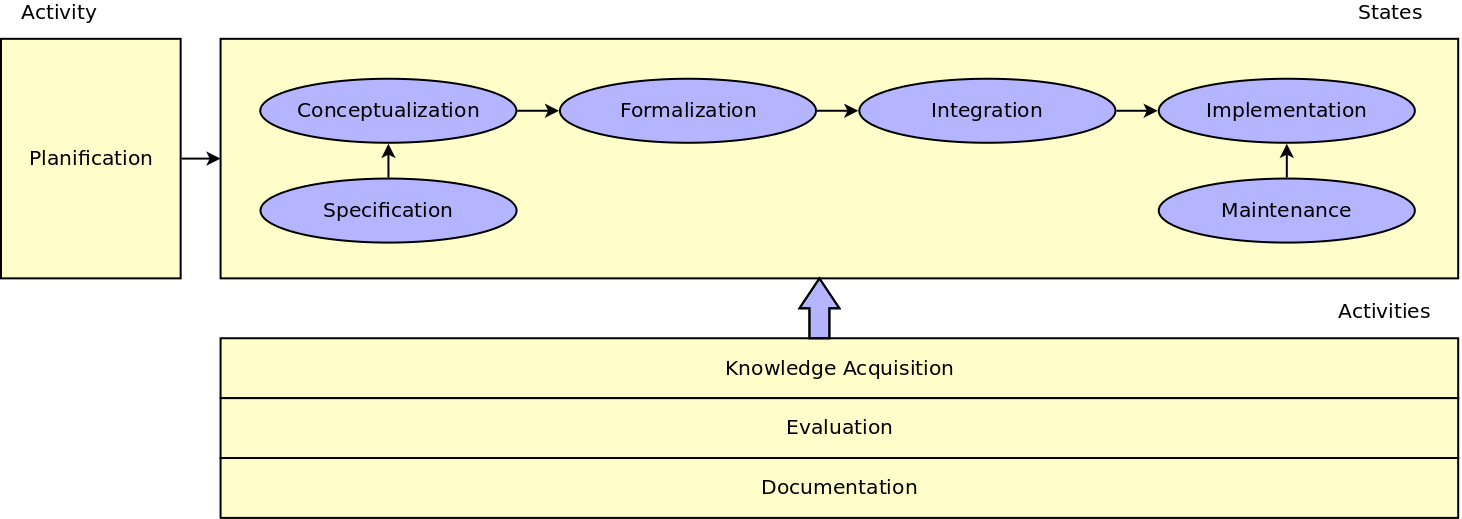
\includegraphics[width=\textwidth]{figures/ontology_lifecycle.pdf}
  \caption{States and activities in the life cycle of an ontology according to \methontology \cite{Methontology}}
  \label{fig:methontology1}
\end{figure}

These activities -- which are depicted in figure \ref{fig:methontology1} -- are arranged into the step of \emph{planification} that must be performed at the very beginning of development, a \emph{set of stages} (consisting of \emph{specification}, \emph{conceptualization}, \emph{formalization}, \emph{integration}, \emph{implementation} and \emph{maintenance}) through which the ontology moves during its creation and some activities (\emph{knowledge acquisition}, \emph{documentation} and \emph{evaluation}) that are performed throughout the whole development process in parallel to the stages.

% TODO figure: evolving life-cycle
Differently to what is shown in figure \ref{fig:methontology1}, \methontology follows an evolving life cycle model similar to the iterative-incremental approach that is used in the \emph{Spiral Model} in software development\cite{spiral_model}. This life cycle model which allows the ontology to grow according to its needs. Whenever it is necessary, pieces of the ontology can be added, modified and deleted. Thus, one state does not have to be completely finished before the next state is begun. The ontology will cycle through each state numerous times until the ontology meets all requirements and the results of each step correspond to each other.

\subsection{METHONTOLOGY}
\label{sec:methontology}

This section describes \methontology as a well-defined approach to perform all activities mentioned above.

For each of the activities, only ideas behind them are covered, but their application is omitted. They are applied in chapter \ref{ch:thinkhomeweather_ontology} where \methontology is used to create the \thinkhomeweather ontology.

Each section that describes an activity that involves the creation of some documentation artefact (e.g. a table or a document), a template for the respective artefact is presented.

\subsubsection{Specification}

\methontology defines a precise approach for the development of an ontology. It specifies certain activities that need to be performed, how these activities are performed and in which order. Thus, the activity of \emph{planification} is completed by specifying \methontology itself and the ontology developer is exempted therefrom. Hence, the first step of developing an ontology from scratch is \emph{specification}

During \emph{specification}, an \emph{Ontology Requirements Specification Document} is generated. This document is written in natural language using a set of intermediate representations or using competence questions. It should include

\begin{itemize} % TODO adapt?
  \item the purpose of the ontology, its intended uses, scenarios of use, end-users etc.,
  \item the level of formality (highly informal, semi-informal, semi-formal or rigorously formal). % TODO reference to Uschuld & Gruninger 1996
  \item the scope which includes the set of terms to be represented, its characteristics and its granularity.
\end{itemize}

A good ontology specification document has the following properties:

\begin{itemize}
  \item \textbf{Consision}: Every term is relevant and there are no duplicated or irrelevant terms.
  \item \textbf{Partial completeness}: % TODO specify?
  \item \textbf{Consistency}: All terms and their meanings make sense in the domain.
\end{itemize}

Below there is a template of an \emph{Ontology Requirements Specification Document}\cite{ORSD}:

\vspace{.5cm}

% TODO ensure there are no page breaks inside this box
\begin{mdframed}[linewidth=.6pt]
\setlength{\parindent}{0pt}
\vspace{.4cm}

\MakeUppercase{\textbf{Ontology Requirements Specification Document}}

\vspace{.6cm}

\textbf{Name}: …

\vspace{.3cm}

\textbf{Purpose}: …

\vspace{.3cm}

\textbf{Scope}: …

\vspace{.3cm}

\textbf{Implementation language}: …

\vspace{.3cm}

\textbf{Intended end-users}: …

\vspace{.3cm}

\textbf{Intended uses}: …

\vspace{.3cm}

\textbf{Ontology requirements}: …

\vspace{.3cm}

\setlength{\leftskip}{.5cm}

\textbf{Non-functional requirements}: 

\begin{itemize}
  \item …
\end{itemize}

\textbf{Functional requirements}: 

\begin{itemize}
  \item …
\end{itemize}

\setlength{\leftskip}{0cm}

\vspace{.2cm}

\textbf{Pre-glossary of terms}: …

\setlength{\leftskip}{0cm}

\end{mdframed}

% \vspace{.5cm}

\subsubsection{Knowledge Acquisition}

Most of knowledge acquisition is done simultanously with the \emph{specification} phase. It is one of the most important activities and needs to be performed thoroughly as most other activities depend heavily on it.

Sources of knowledge are experts, books, handbooks, figures, tables and even other ontologies. Knowledge will be collected using techniques such as brainstorming, interviews, formal and informal analysis of texts and knowledge acquisition tools.

\subsubsection{Conceptualization}

% TODO placement?
\begin{figure}
  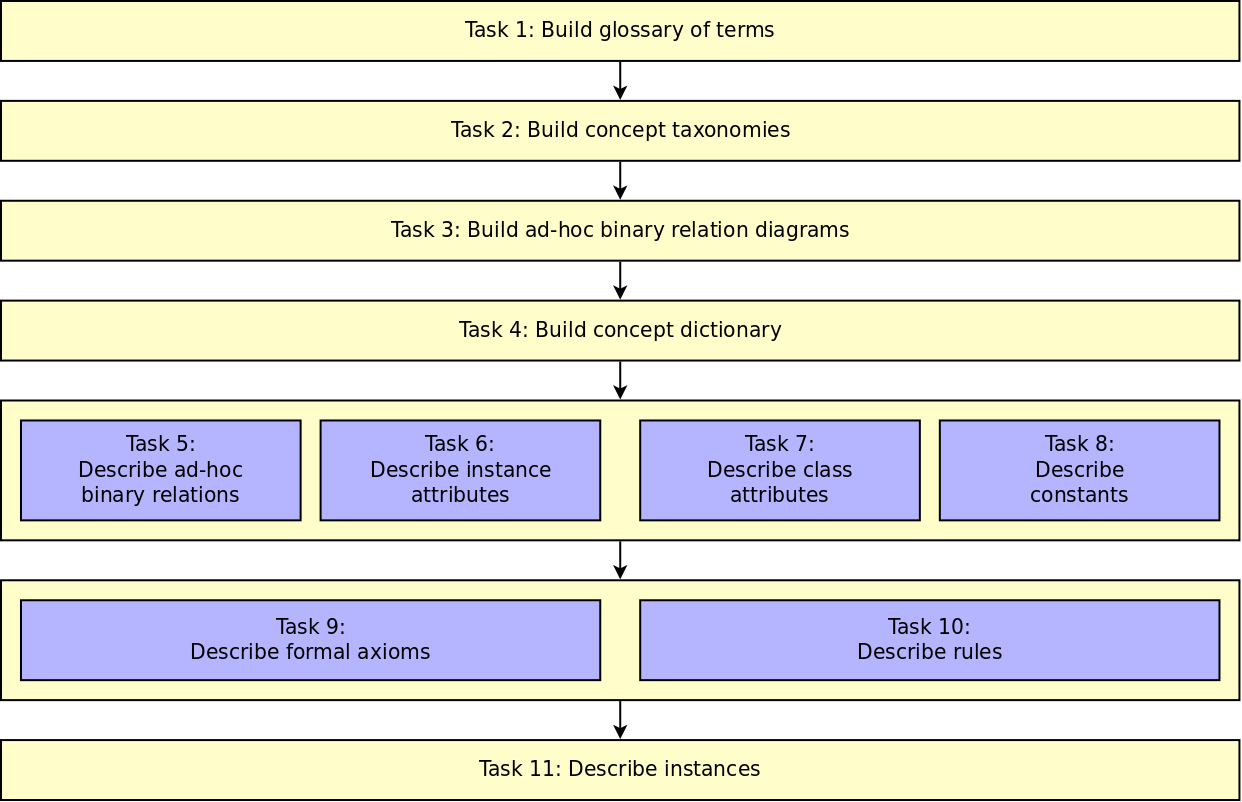
\includegraphics[width=\textwidth]{figures/methontology_tasks.pdf}
  \caption{Tasks of the conceptualization activity according to \methontology \cite{MethontologyLegal}}
  \label{fig:methontology2}
\end{figure}

The state of \emph{conceptualization} consists of several tasks as shown in figure \ref{fig:methontology2} \cite{MethontologyLegal}. Again, the figure shows the tasks in a sequential manner. However, as \methontology uses an evolutional process model, the steps will be performed numerous times.

% TODO templates for each table
% TODO these sections do not relate to the sections in the next chapter?!
\paragraph{Task 1: Glossary of Terms}

At first, the ontologist builds a \emph{Glossary of Terms}. This glossary includes all the relevant terms of the domain (concepts, instances, attributes, relations etc.). It can be built as a table having the columns \emph{name}, \emph{synonyms}, \emph{acronyms}, \emph{description} (for a natural language description of the term) and \emph{type} (specifying whether the term is a concept, an instance, an attribute, a relation etc.).

\begin{figure}
\centering
\begin{tabular}{|p{.2\textwidth}|p{.2\textwidth}|p{.2\textwidth}|p{.2\textwidth}|}
  \hline
  \textbf{Name} & \textbf{Acronyms} & \textbf{Description} & \textbf{Type} \\
  \hline\hline
  … & … & … & … \\
  \hline
\end{tabular}
\caption{Template for the glossary of terms as proposed by \methontology.}
\label{fig:methontology_example_glossary}
\end{figure}

Figure~\ref{fig:methontology_example_glossary} shows a template for the glossary of terms.

\paragraph{Task 2: Concept Taxonomies}

When the glossary of terms contains a sizable number of concepts, these ontologies will be arranged one or more taxonomies that define the concept hierarchy. It is advisable to display the taxonomies in several diagrams.

% TODO reference Frame Ontology and OKBC Ontology
\methontology proposes the use of four taxonomic relations:
% TODO description
\begin{enumerate}
  \item \textbf{Subclass-Of}
  \item \textbf{Disjoint-Decomposition}
  \item \textbf{Exhaustive-Decomposition}
  \item \textbf{Partition}
\end{enumerate}

% TODO error check?

\begin{figure}
\centering
\includegraphics[width=.9\textwidth]{figures/diagrams/methontology_example_concept_taxonomies.pdf}
\caption{Example of a concept-classification tree as proposed by \methontology.}
\label{fig:methontology_example_concept_taxonomies}
\end{figure}

The concept taxonomies are visualised in \emph{concept-classification trees} which are diagrams that depict the concepts and their taxonomic relations. See figure~\ref{fig:methontology_example_concept_taxonomies} for an example of a concept-classification trees. In case the ontology contains a large number of concepts, the tree may be split into several diagrams.

\paragraph{Task 3: Ad-hoc binary relation diagrams}

In the next step, \emph{ad-hoc binary relation diagrams} are created. This diagrams show all ad-hoc relationships between concepts of the same (or different) concept taxonomy. Figure~\ref{fig:methontology_example_binary_relations} for an example of a binary relation diagram.

\begin{figure}
\centering
\includegraphics[width=.8\textwidth]{figures/diagrams/methontology_example_binary_relations.pdf}
\caption{Example of a binary relations diagram as proposed by \methontology.}
\label{fig:methontology_example_binary_relations}
\end{figure}

% TODO error check

\paragraph{Task 4: Concept dictionary}

The \emph{concept dictionary} contains all domain concepts together with their relations, their instances and their class and instance attributes. All information from the previous steps contribute to this dictionary. It is again be built as a table having appropriate columns. Like the concept-classification trees, this table may be split into a set of smaller tables if the ontology contains a large number of concepts.

\begin{figure}
\centering
\begin{tabular}{|p{.2\textwidth}|p{.5\textwidth}|p{.2\textwidth}|}
  \hline
  \textbf{Name} & \textbf{Instances} & \textbf{Relations} \\
  \hline\hline
  … & … & … \\
  \hline
\end{tabular}
\caption{Template for the concept dictionary as proposed by \methontology.}
\label{fig:methontology_example_concept_dictionary}
\end{figure}

Figure~\ref{fig:methontology_example_concept_dictionary} shows a template for the concept dictionary.

% TODO error check

\paragraph{Task 5: Ad-hoc binary relation details}

In this step, for all ad-hoc binary relations details will be specified in a tabular manner. The resulting table will have a row for each relation and columns named \emph{relation name}, \emph{source concept}, \emph{source cardinality (max)}, \emph{target concept}, \emph{inverse relation}.

% TODO error check

\begin{figure}
\centering
\begin{tabular}{|p{.167\textwidth}|p{.167\textwidth}|p{.167\textwidth}|p{.167\textwidth}|p{.167\textwidth}|}
  \hline
  \textbf{Name} & \textbf{Source\newline concept} & \textbf{Target\newline concept} & \textbf{Maximum\newline source\newline cardinality} & \textbf{Inverse\newline relation} \\
  \hline\hline
  … & … & … & … & … \\
  \hline
\end{tabular}
\caption{Template for the binary relations table as proposed by \methontology.}
\label{fig:methontology_example_binary_relations_table}
\end{figure}

Figure~\ref{fig:methontology_example_binary_relations_table} shows a template for the binary relations table.

\paragraph{Task 6: Instance attributes}

This step leads to an \emph{instance attributes table}. That is a table of all \emph{instance attributes} that are listed in the concept dictionary. Each row contains the description of one instance attribute. An instance attribute is an attribute that describes an instance of a concept. Its value may be different for each instance of the concept. The columns of the table are \emph{attribute name}, \emph{concept name}, \emph{value type} (\emph{Integer}, \emph{Float}, \emph{String}, etc.), \emph{value range}, \emph{minimum cardinality} and \emph{maximum cardinality}. Additionally, the following information may be specified: instance attributes, class attributes and constants used to infer values of the attribute; attributes that can be inferred using values of this attribute; formulae or rules that allow inferring values of the attribute; and references used to define the attribute.

\begin{figure}
\centering
\begin{tabular}{|p{0.15\textwidth}|p{0.15\textwidth}|p{0.15\textwidth}|p{0.15\textwidth}|p{0.15\textwidth}|p{0.15\textwidth}|}
  \hline
  \textbf{Attribute name} & \textbf{Concept name} & \textbf{Value type} & \textbf{Value range} & \textbf{Unit} & \textbf{Cardinality} (min, max)\\
  \hline\hline
  … & … & … & … & … & … \\
  \hline
\end{tabular}
\caption{Template for the instance attributes table as proposed by \methontology.}
\label{fig:methontology_example_instance_attributes}
\end{figure}

See figure~\ref{fig:methontology_example_instance_attributes} for a template for the instance attributes table.

\paragraph{Task 7: Class attributes}

All class attributes that are listed in the concept dictionary are described in detail in the \emph{class attributes table}. Each row describes one class attribute. The columns will be \emph{name}, \emph{concept name} (i.e. the name of the concept where the attribute is defined), \emph{value type}, \emph{value(s)}, \emph{minimum cardinality} and \emph{maximum cardinality}. Additionally, all information about related instance attributes, class attributes, constants, rules and formulae may be specified that are specified in the instance attribute as well.

\begin{figure}
\centering
\begin{tabular}{|p{0.22\textwidth}|p{0.22\textwidth}|p{0.22\textwidth}|p{0.22\textwidth}|}
  \hline
  \textbf{Super-concept} & \textbf{Sub-concept} & \textbf{attribute name} & \textbf{attribute value(s)} \\
  \hline\hline
  … & … & … & … \\
  \hline
\end{tabular}
\caption{Template for the class attributes table as proposed by \methontology.}
\label{fig:methontology_example_class_attributes}
\end{figure}

Figure~\ref{fig:methontology_example_class_attributes} shows a template for the class attributes table.

\paragraph{Task 8: Constants}

In this step, the \emph{constants table} is created that specifies details about all the constants listed in the glossary of terms. For each constant the following is specified: name, value type, value, the measurement unit for numerical constants and the attributes that can be inferred using the constant.

% TODO constants table -> instances table?
\begin{figure}
\centering
\begin{tabular}{|p{0.2\textwidth}|p{0.2\textwidth}|}
  \hline
  \textbf{Instance name} & \textbf{Concept name} \\
  \hline\hline
  … & … \\
  \hline
\end{tabular}
\caption{Template for the constants table as proposed by \methontology.}
\label{fig:methontology_example_constants}
\end{figure}

Figure~\ref{fig:methontology_example_constants} shows a template for the constants table.

\paragraph{Task 9: Formal axioms}

% TODO

% TODO template

\paragraph{Task 10: Rules}

% TODO

% TODO template

\paragraph{Task 11: Instances}

% TODO

\subsubsection{Integration}

As ontologies are built for reuse and the wheel shall not be reinvented during the creation of a new ontology, the ontologist searches for existing ontologies. The goal is to import ontologies that already define terms that are part of the conceptualization of the ontology currently being developed.

\subsubsection{Implementation}

% TODO references
The task of implementation requires an environment that supports the ontologies selected in the integration step. Features that should be provided by such an environment are

% TODO make description more detailled?
\begin{itemize}
  \item a lexical and syntactic analyzer to guarantee the absence of lexical and syntactic errors,
  \item an editor for adding, modifying and removing definitions,
  \item a browser for inspecting the library of ontologies and their definitions,
  \item a searcher for looking for the most appropriate definitions,
  \item evaluators for detecting incompleteness, inconsistencies and redundant knowledge and
  \item an automatic maintainer for managing the inclusion, removal or modification of existing definitions.
\end{itemize}

In the case of the \thinkhomeweather ontology an \eacs{OWL} ontology is created using \protege together with the Pellet reasoner.

\subsubsection{Evaluation}

% TODO

\subsubsection{Documentation}

% TODO citation: problems with documentation after development

During the steps described above, a set of documents is compiled. If generated properly and accurately, these documents describe every detail of the ontology. Using this approach, \methontology forces the ontology designer to document throughout the development process. Any problems that come with documentation being created after the development process -- e.g. incomplete or wrong documentation, the ontology designer does not write the documentation herself, or some ideas the designer had in the design process are lost -- are avoided.

Hence, in \methontology, \emph{documentation} is an activity that is not performed explicitely. One the development process has finished, both the ontology and its documentation are ready to use. 

\subsubsection{Maintenance}

At any time in the future, changes to the ontology may become necessary. A modification of the ontology's requirements may be one reason therefor; inaccurateness that occurs during the ontology development process may be another reason.

Whenever a change is necessary, the ontology again cycles the states of \emph{specification}, \emph{conceptualization}, \emph{formalization}, \emph{integration} and \emph{implementation} repeatedly until all requirements are met and all artefacts generated in these states correspond to each other. \emph{Knowledge acquisition} and \emph{evaluation} are again performed throughout all of these states.

